%----------------------------------------------------------------------------------------
%	PACKAGES AND DOCUMENT CONFIGURATIONS
%----------------------------------------------------------------------------------------
\documentclass[11pt]{article}
\usepackage{amsmath} % Required for some math elements
\usepackage{hyperref} 
\usepackage{xcolor}
\usepackage{lipsum} 
\usepackage{cite}
\usepackage{graphicx} % Required for the inclusion of images
\usepackage{algorithmic}
\usepackage{array}
\usepackage{bookmark}
\usepackage{listings}
\usepackage{amssymb}
\usepackage{enumitem}
\usepackage[margin=24mm]{geometry}
\usepackage[caption=false, font=footnotesize]{subfig}

\newlist{steps}{enumerate}{1}
\setlist[steps, 1]{label = Step \arabic*:}

\hypersetup{ %color attributes of citation, link, etc.
    colorlinks=true,
    linkcolor=blue,
    filecolor=gray,      
    urlcolor=blue,
    citecolor=blue,
}

\newcommand{\matlab}{\textsc{Matlab }} %very important and totally necessary addition

\newcommand\Item[1][]{%
  \ifx\relax#1\relax  \item \else \item[#1] \fi
  \abovedisplayskip=0pt\abovedisplayshortskip=0pt~\vspace*{-\baselineskip}}
%----------------------------------------------------------------------------------------
%	DOCUMENT INFORMATION
%----------------------------------------------------------------------------------------
 
\title{ENGR 222 \\ Assignment 1 Submission}
\author{Daniel Eisen : 300447549}
\date{\today}

\begin{document}
\maketitle
%----------------------------------------------------------------------------------------
%	DOCUMENT CONTENT
%----------------------------------------------------------------------------------------
\begin{enumerate}
    \item Consider the parametric equations:
    $(x,y) = (8sin(t),2t-sin(2t))$
    \begin{enumerate}
        \Item 
        \begin{align*}
            (x,y) = [&(0,0),(5.657,0.571),(8,\pi),(5.657,5.712),(0,2\pi),\\
                  &(-5.657,6.854),(-8,3\pi),(-5.657,11.996),(0,4\pi)]
        \end{align*}

        \begin{center}
            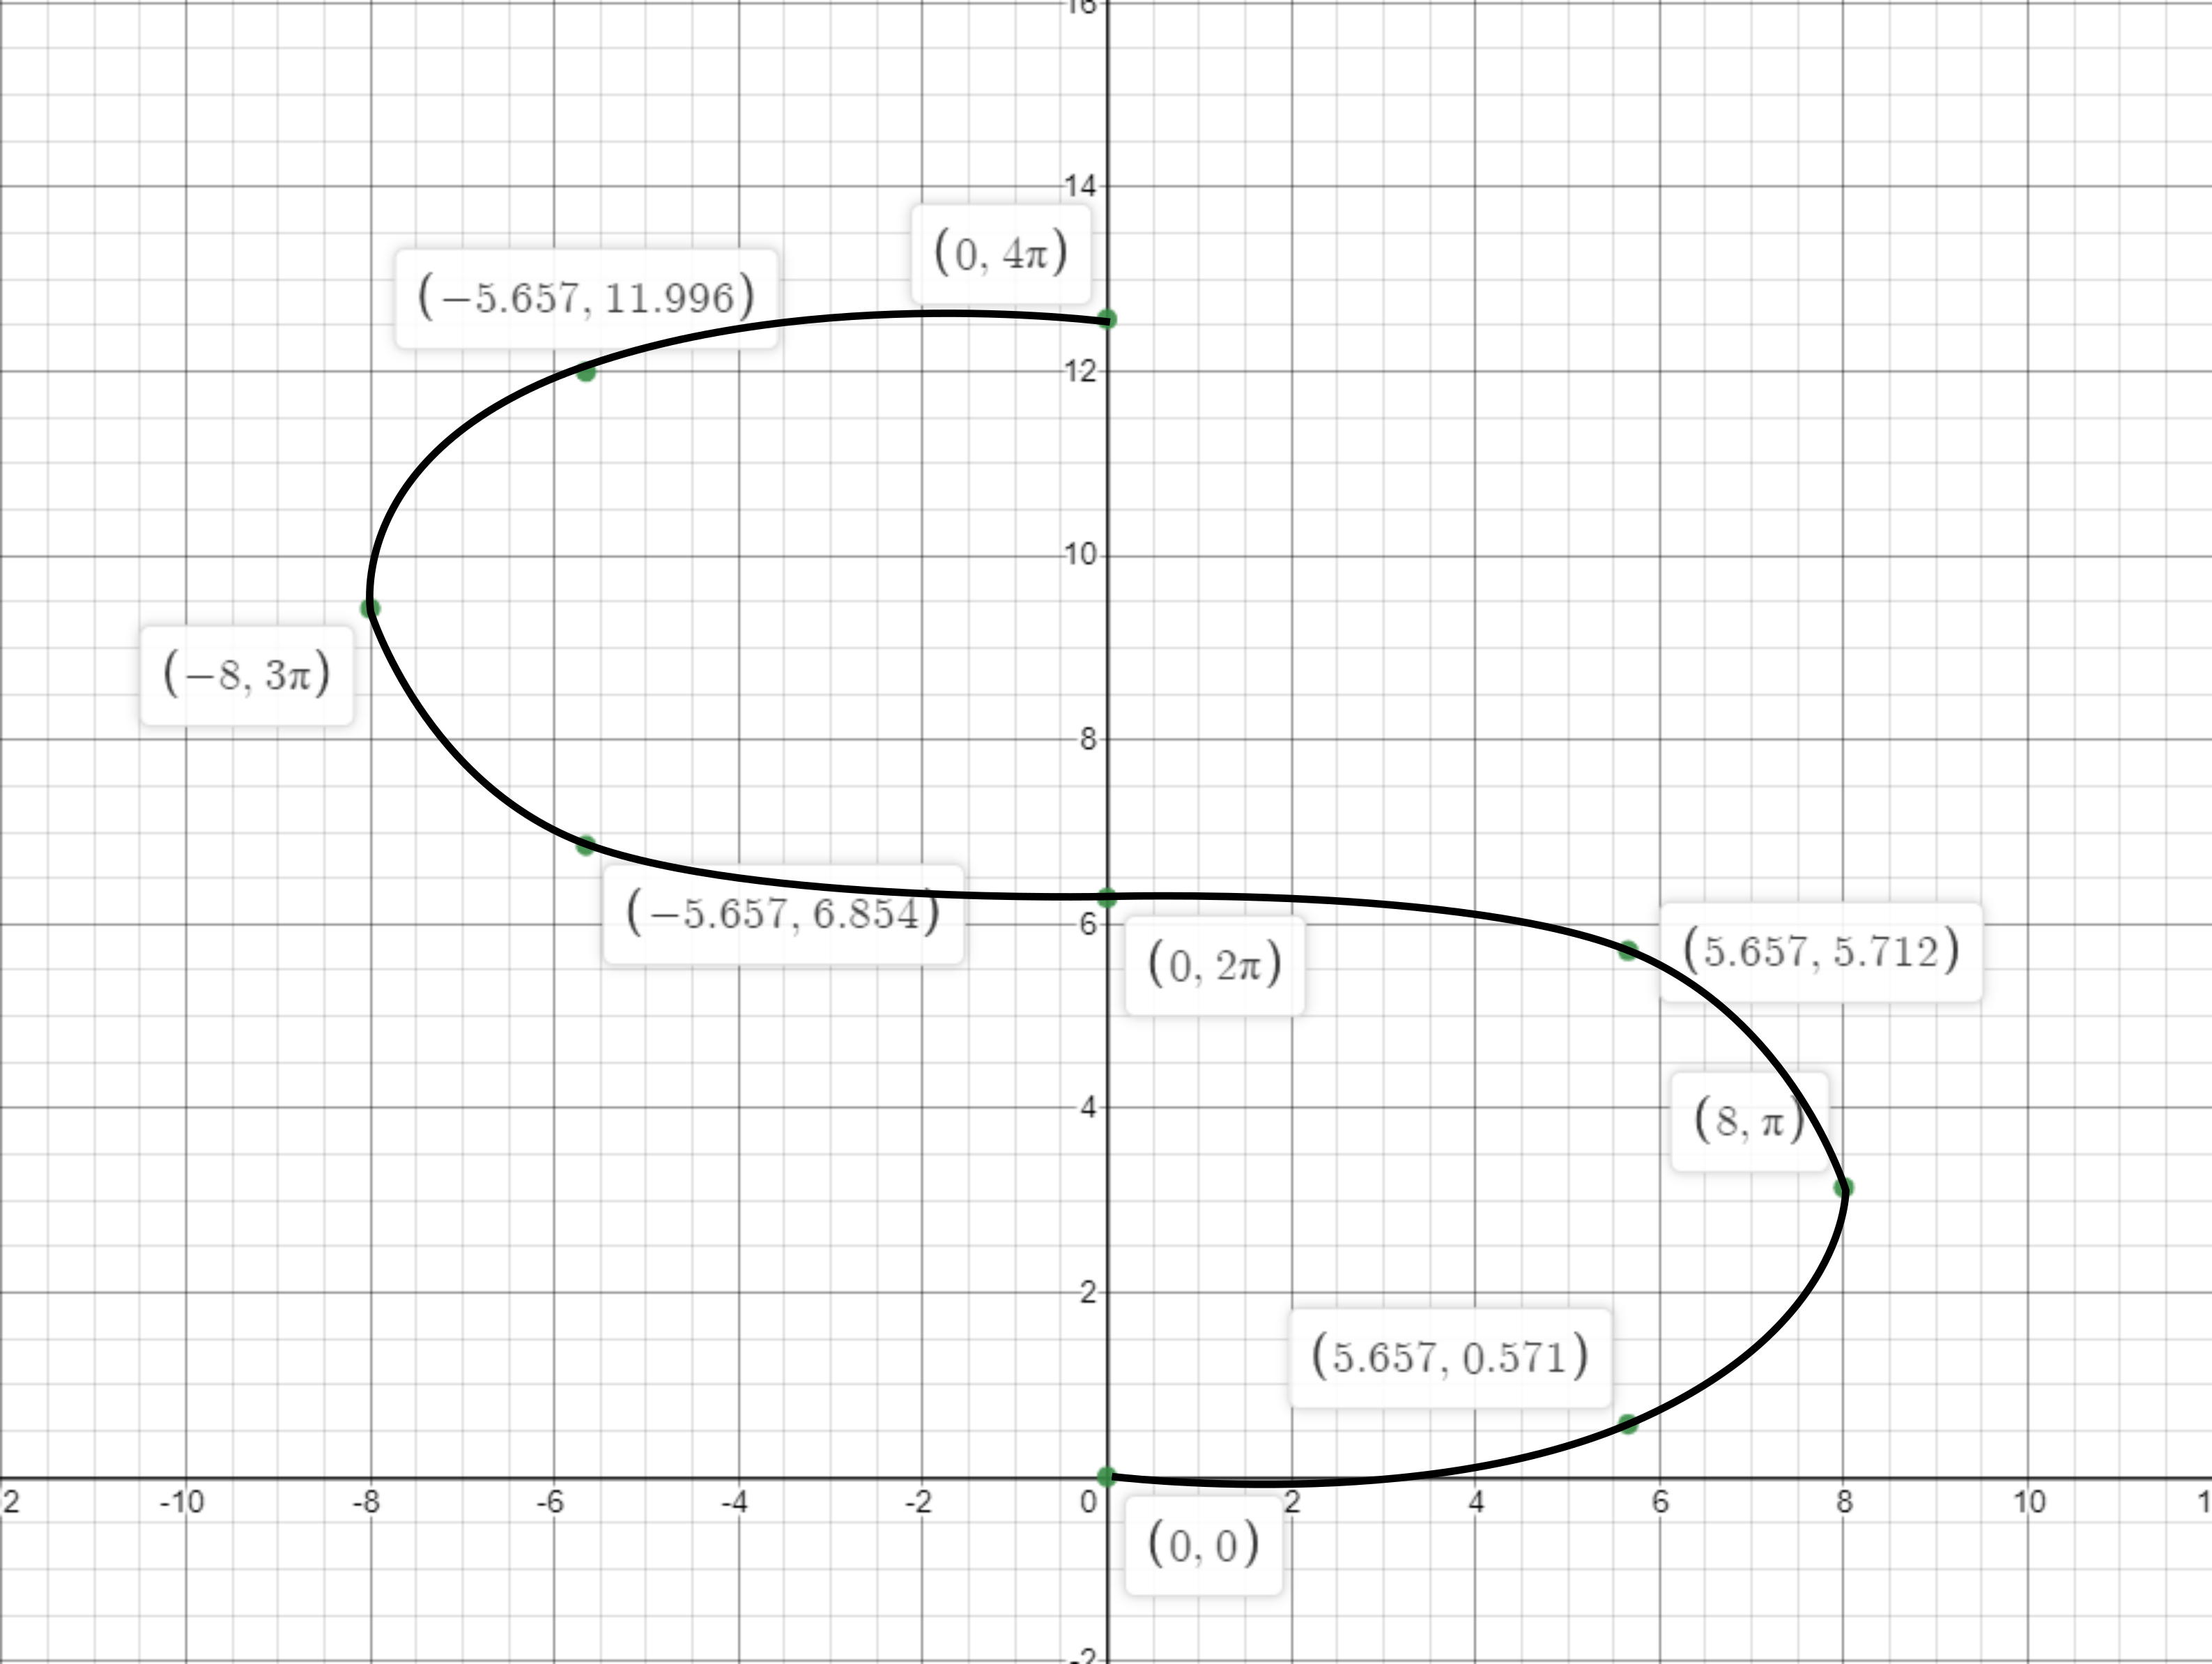
\includegraphics[width=0.4\textwidth]{inc/1a.png}
        \end{center}

        \Item
        \begin{align*}
            \frac{d}{dt}(x,y) &= (8cos(t), 2 - 2cos(2t))\\
            t=\pi/6 \;:\; \frac{d}{dt}(x,y) &= (6.928203,1)\\
        \end{align*} 
        Unit tangent vector:
        \begin{align*}
           \frac{\frac{d}{dt}(x,y)}{\| \frac{d}{dt}(x,y) \|} = \frac{(6.928203,1)}{\sqrt{6.928203^2+1}} = \left(\frac{6.928203}{7},\frac{1}{7}\right) 
        \end{align*}
        \Item
        \begin{align*}
            &= (x,y) + t{\cdot} \frac{\frac{d}{dt}(x,y)}{\| \frac{d}{dt}(x,y) \|}\\
            &= (4,0.181) + t\left(\frac{6.928203}{7},\frac{1}{7}\right)\\
            &= \left(\frac{6.928203t}{7}+4,\frac{t}{7}+0.181)\right)
        \end{align*} 
        \Item 
        Normal line:
        \begin{align*}
            &= \left( f(\frac{\pi}{6}) - tg'(\frac{\pi}{6}), g(\frac{\pi}{6}) + tf'(\frac{\pi}{6}) \right) \\
            &= \left( 4 - t, 0.181 + 6.928203t \right)
        \end{align*}
        \item 
    \end{enumerate}
    \item Consider the curve described by the vector valued function:
    \begin{enumerate}
        \item 
        \item 
        \item 
        \item 
        \item 
    \end{enumerate}
    \item Quick questions:
    \begin{enumerate}
        \item 
        \item 
        \item  
        \item  
        \item  
    \end{enumerate}
    \item Suppose a roller coaster path described by:
    \begin{enumerate}
        \item 
        \item 
        \item  
        \item  
        \item  
    \end{enumerate}
\end{enumerate}


\end{document}